%!TEX root = ../memoria.tex

\chapter{Modelo de desarrollo}

\section{Elección del modelo}

Para el desarrollo de la presente aplicación será empleada \emph{Extreme Programming (XP)} que corresponde a una de las metodologías basadas en el manifiesto ágil \footnote{http://agilemanifesto.org/iso/es/manifesto.html}. Bajo la lógica de un desarrollo iterativo e incremental se desarrollará la aplicación en ciclos o iteraciones que añaden funcionalidades al sistema, comenzando por los requerimientos más críticos o básicos.

Debido a la naturaleza de la aplicación (enfocada a servicios), el desarrollo iterativo se adapta muy bien al proceso de creación del sistema. Esto debido a que las distintas funcionalidades de la aplicación pueden ser desarrolladas de forma individual unas de otras y en iteraciones distintas. El segundo principio del desarrollo ágil\footnote{http://agilemanifesto.org/iso/es/principles.html} toma una importancia vital en la creación de funciones que pueden ser \emph{testeables} en etapas tempranas del proyecto. 

Según lo dicho anteriormente, la frase apócrifa \emph{divide et impera} toma relevancia al dividir el problema completo en tres módulos e incluso en funciones encapsuladas que pueden ser desarrolladas de forma individual.

La capacidad iterativa de las metodologías agiles se complementa con la posibilidad de desarrollar funciones de forma paralela, de este modo se puede reducir el tiempo de desarrollo entre iteraciones. Si bien, esta característica no es aplicable a la totalidad del proyecto si puede ser aplicada a funciones que no tengan una dependencia de otras. 

Hasta el momento se han nombrado dos ventajas propias de todas las metodologías que sigan la lógica del desarrollo ágil. \emph{Extreme Programming} entrega ventajas propias que se adaptan a lo esperado y aseguran un \emph{software} de calidad. 

Las pruebas unitarias continuas, facilitadas por el desarrollo iterativo permiten probar funcionalidades completas de forma temprana y a su vez, la corrección temprana en caso de identificar fallas.

El \emph{Test-Driven Development (TDD)} corresponde a un \emph{framework} de \emph{Extreme Programming} que se basa en la definición de pruebas unitarias antes del desarrollo de la aplicación y la implementación de estas en paralelo al trabajo de codificación del sistema, de este modo aseguramos el cumplimiento de los requerimientos definidos con el cliente. Es importante notar que el proceso de pruebas unitarias de las funciones terminadas y el desarrollo de otras iteraciones puede ser gestado en paralelo permitiendo reducir el tiempo de desarrollo sin desmedro de la calidad final del \emph{software}. 

Test-Driven Development sigue la siguiente estructura:
\begin{itemize}
	\item Diseño de la arquitectura de alto nivel.
	\item Codificación
		\begin{itemize}
		\item Prueba unitaria
		\item Codificación
		\item Refactorización
		\end{itemize}
	\item Testing
\end{itemize}

\begin{figure}[ht!]
\centering
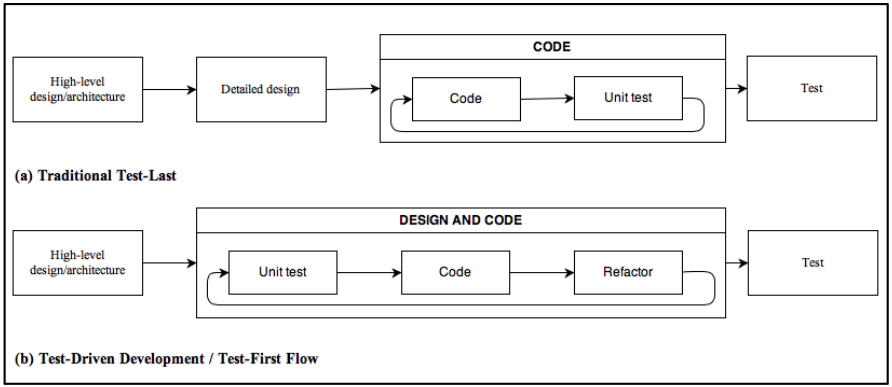
\includegraphics[width=1\textwidth]{figures/mapa-tdd.png}
\caption{Model of Janzen and Saiedian (2008) - Traditional Development vs. TDD}
\label{fig:Traditional Development vs. TDD}
\end{figure}

La figura \ref{fig:Traditional Development vs. TDD} muestra la secuencia de los procesos según \emph{Test-Driven Development} (a) en contraposición con la secuencia tradicional (b).

En base a la metodología seguida, los comentarios dentro del código son esenciales para una buena refactorización de este, permitiendo que sea legible. Como fue explicado, debido al ciclo continuo de prueba, codificación y refactorización es necesaria una rápida comprensión del algoritmo y su funcionalidad. Esta secuencia cíclica facilita reescribir el código de una mejor forma, optimizando no solo el funcionamiento de este si no que eliminando bloques innecesarios o duplicados.

Por otro lado, una de las desventajas de emplear \emph{TDD} es que debido a su lógica de diseño emergente carece de un esquema de diseño detallado del sistema completo, que podría ser obtenido con otras metodologías, como por ejemplo, un enfoque de diseño orientado a objetos (\emph{OOD}).  Para el caso particular de \emph{Gerprin}, no es un punto crucial, debido a que el sistema fue desarrollado con anterioridad y se conocen las interacciones entre los módulos y las funciones que los componen de sobremanera.

\section{Definición de actividades}

El ciclo de vida de un proyecto desarrollado empleando XP está compuesto de seis fases\footnote{http://www.cyta.com.ar/ta0502/v5n2a1.htm}:  

\begin{enumerate}
	\item Exploración
	\item Planificación de las entregas
	\item Iteraciones
	\item Integración y pruebas
	\item Aceptación y entrega
	\item Muerte del proyecto
\end{enumerate}

\subsection{Exploración}

Exploración es la actividad inicial del ciclo de vida del desarrollo de un proyecto empleando \emph{XP} como metodología. Consiste en la realización de las primeras interacciones con el proyecto, tomando conocimiento en líneas generales de las historias de usuario del \emph{software} a desarrollar. 

Es importante en esta etapa definir las herramientas, metodologías, canales de comunicación y \emph{framework} que se utilizaran, además, realizar un primer acercamiento de estas al equipo de trabajo, para familiarizarse con su uso.

\subsection{Planificación de las entregas}

En la etapa de planificación de la entrega se deben definir las prioridades de las historias de usuario y el esfuerzo que debe ser empleado en el desarrollo de dicha historia. Lo anterior, con el objetivo de determinar el orden y contenido de los entregables.

Para lo anterior se debe elaborar un informe con las historias de usuario que serán desarrolladas en cada entregable y la estimación del tiempo que tardará en ser completado. El documento debe definir la fecha de finalización de cada una de las iteraciones programadas separadas en plazos de no más de tres semanas. 

Esta etapa se debe repetir antes de cada iteración para definir el contenido del siguiente entregable y corregir, de ser necesario, las estimaciones realizadas en iteraciones anteriores.

Con el fin de obtener una retroalimentación del tiempo de trabajo y poder corregir a tiempo problemas de atraso que se estén produciendo, se empleará un sistema de puntaje para medir el tiempo de desarrollo de las historias donde un punto equivale a una semana de trabajo de una persona. De este modo cada historia tiene un estimado de trabajo y el valor real de la labor realizada, buscando que dichos valores sean lo más similar posible

\subsection{Iteraciones}

Las iteraciones corresponden a varias entregas que se realizan de forma periódica basadas en el documento generado en la etapa anterior.

En la primera iteración se debe realizar un diseño de la arquitectura del sistema, definiendo a grandes rasgos la relación entre las partes que lo componen. Lo anterior se logra realizando un breve análisis de las historias de usuario que fuercen el uso de una arquitectura especifica. 

Debido a que la lógica de trabajo se basa en diseño emergente, no es necesario un gran detalle en el diseño, esto debido a que se debe consdierar que dicho diseño puede verse afectado por futuras decisiones en el desarrollo.

En esta etapa se adopta el flujo de trabajo de \emph{TDD}, donde antes de comenzar los trabajos de programación se escriben las pruebas unitarias que deben ser aprobadas por los distintos procesos a desarrollar. Dichas pruebas deben ser realizadas en paralelo a la codificación del programa, de esta forma, cada prueba da lugar a una refactorización del código, permitiendo que el diseño emerja desde la optimización del mismo.

Para comprender de una mejor forma esta lógica de trabajo se debe entender que cada prueba que dé a conocer un error del programa es una prueba exitosa, esto debido a que nos permite conocer los errores antes de que estos pacen al proceso de producción. 

\subsection{Integración y pruebas}

La etapa de Integración y pruebas consiste en la instalación de la aplicación en su ubicación final, donde se realizarán pruebas de integración que permiten comprobar que las configuraciones y relaciones entre las partes del sistema funcionen correctamente. 

Junto con lo anterior, se deben considerar nuevas funcionalidades para la aplicación que no fueron incluidas en las fases anteriores y que son deseables para nuevas versiones.

\subsection{Aceptación y entrega}

Para esta etapa la aplicación debe ser entregada mientras se encuentra en los servidores de producción, con el objetivo de resolver situaciones que presentaron problemas en las pruebas de integración y desarrollar las funcionalidades que fueron solicitadas en la etapa anterior. 

\subsection{Muerte del proyecto}

Debido a que el proyecto no recibirá más cambios, en esta etapa se debe desarrollar un manual de usuario explicando las funcionalidades del sistema que contenga el propósito de cada función, como usarlas correctamente, los valores configurables, su significado y las restricciones de estos.

Además, se deberá realizar un documento de diseño de la arquitectura final del sistema con el propósito de documentar el funcionamiento de este en caso de futuras mejoras. 

\section{Productos de Trabajo}

El manifiesto ágil, en el segundo elemento que se ha aprendido a valorar dice “Software funcionando sobre documentación extensiva”. Debido a esto los productos de trabajo generados por cada una de las etapas van enfocadas a un software funcional más que a la documentación.

Sin embargo, el mismo manifiesta concluye “aunque valoramos los elementos de la derecha (documentación), valoramos más los de la izquierda (código funcionando)”. Los productos de trabajo que no corresponden a código funcional, es decir, corresponden a documentos, planes de trabajo, manuales o especificaciones deben encontrarse en proporción al trabajo a realizar.

A continuación, se detallan los productos de trabajo que deben ser generados:

\begin{enumerate}
	\item Especificación de Requerimientos
	\item Planificación de proyecto
	\item Plan de pruebas
	\item Especificación del Sistema
	\item Plan de Aseguramiento de Calidad (\emph{SQA})
	\item Manual de usuario
\end{enumerate}

\subsection{Especificación de Requerimientos}

Para comprender de mejor forma el sistema que se busca construir, es necesario realizar un proceso de documentación esquemática de los requerimientos que forman parte del sistema.

La especificación de requerimiento es un documento que mediante la declaración y definición de los requerimientos funcionales y no funcionales del sistema describe el comportamiento completo de este.

Basado en \citet{mem00}, el siguiente esquema muestra el índice de contenidos del documento. 

\vspace{10mm}
\begin{framed}
     \begin{enumerate}
		\item \textbf{Introducción}
		\begin{enumerate}
			\item Propósito del documento
			\item Alcance del producto
			\item Definiciones, acrónimos y abreviaturas
			\item Referencias
			\item Descripción del resto del documento
		\end{enumerate}
		\item \textbf{Descripción general}
		\begin{enumerate}
			\item Perspectiva del producto
			\item Funciones del producto
			\item Características del usuario
			\item Restricciones generales
			\item Suposiciones y dependencias
		\end{enumerate}		
		\item \textbf{Requerimientos Específicos}

		Incluye los requerimientos funcionales, no funcionales y de interfaz. Obviamente esta es la parte más sustancial del documento, pero debido a la amplia variedad en la práctica organizacional, no es apropiado definir una estructura estándar para esta sección. Los requerimientos pueden documentar las interfaces externas, describir la funcionalidad y el rendimiento del sistema, especificar los requerimientos lógicos de la base de datos, las restricciones de diseño, las propiedades emergentes del sistema y las características de calidad.
		\item \textbf{Apéndice}
		\item \textbf{Índice}
	\end{enumerate}
\end{framed}

\subsection{Planificación de proyecto}
Antes de comenzar a escribir código, es necesario planear las distintas entregas y el contenido de estas. El documento debe contener las historias de usuarios que serán incluidas en cada iteración y las fechas de entrega de cada una de estas.

Para lograr establecer una correcta planificación de las iteraciones, se deben escribir todas las historias de usuario del sistema, para luego valorarlas en termino de complejidad e importancia, estableciendo una ruta crítica de las actividades a realizar. 

Se debe notar que debido a las características del trabajo de desarrollo de \emph{software} es necesario ser flexible sobre el contenido de cada entrega, considerando cambios solicitados por el cliente, corregir errores detectados en iteraciones anteriores, entre otras actividades que pueden ser incluidas en iteraciones futuras. Debido a esto es necesario contemplar modificar la planificación con cada nueva iteración.

El esquema muestra el índice de contenido del producto de trabajo, basado en \citet{mem00}

\begin{framed}
     \begin{enumerate}
		\item \textbf{Introducción}
		\begin{enumerate}
			\item Objetivo
			\item Alcance 
		\end{enumerate}
		\item \textbf{Estimación de esfuerzo y duración}
		\begin{enumerate}
			\item Estimación de esfuerzo
		\end{enumerate}		
		\item \textbf{Organización del Proyecto}

		Describe la forma en que el equipo de desarrollo está organizado, la gente involucrada y sus roles.
		\item \textbf{Planificación}

		Descomposición detallada de las actividades. Señala el \emph{hardware} y \emph{software} de ayuda requeridos para llevar a cabo el desarrollo. Describe la división del proyecto en actividades e identifica hitos asociados a cada actividad.
		\item \textbf{Estrategia del seguimiento}
		\item \textbf{Interfaz externa al proyecto}
		\item \textbf{Identificación y análisis de los riesgos}
	\end{enumerate}
\end{framed}

\subsection{Plan de pruebas}

Uno de los ejes fundamentales al trabajar bajo \emph{TDD} son las pruebas constantes que deben ser realizadas para asegurar un correcto funcionamiento. El plan de pruebas, al igual que la planificación de iteraciones, es un documento que sufrirá modificaciones y será escrito a lo largo del desarrollo del proyecto.

Ante de comenzar la labor de codificación de cada iteración, se deben escribir las distintas pruebas que confirmaran la integración y funcionamiento correcto de cada entregable. 

Antes de desarrollar cualquier función se deben establecer las siguientes pruebas. 

\begin{description}
	\item[Pruebas unitarias:]\hfill

	Son pruebas que aseguran el correcto funcionamiento de una unidad específica del sistema. 

	\item[Pruebas de integración:]\hfill

	Pruebas que comprueban que la correcta integración de todos los elementos unitarios que componen el sistema.

	\item[Pruebas de aceptación:]\hfill

	Las pruebas de aceptación son realizadas en la última iteración y prueban el sistema completo antes de ser instalado en ambiente productivo.

	\item[Pruebas de sistema:]\hfill

	Las pruebas de sistema realizan una comparación entre los objetivos originales del sistema, aquellos planteados en la toma de requisitos, y los procesos, actividades y rutinas del sistema desarrollado.
\end{description}

El esquema muestra el índice de contenido del producto de trabajo, basado en \citet{mem00}

\begin{framed}
     \begin{enumerate}
		\item \textbf{Introducción}
		\begin{enumerate}
			\item Objetivo
			\item Alcance 
		\end{enumerate}
		\item \textbf{Definición de elementos a probar}	
		\item \textbf{Definición de la estrategia a utilizar}

		Describe los recursos a emplear. Especificación de técnica que se usará. Herramientas utilizadas. Criterio indicador de éxito de las pruebas.
		\item \textbf{Equipo de pruebas}
	\end{enumerate}
\end{framed}

\subsection{Especificación del Sistema}

Debido a que la labor de \emph{software} es un trabajo realizado en equipo, es necesario dejar plasmada la arquitectura del sistema y explicar a grandes rasgos el funcionamiento de los distintos procesos. Esto con el objetivo de ayudar a futuros desarrolladores que realicen labores de mantención o actualizaciones al sistema.

Las especificaciones del sistema deben contener la arquitectura y descripción de las funciones que componen cada una de las distintas partes.

El esquema muestra el índice de contenido del producto de trabajo, basado en \citet{mem00}

\begin{framed}
     \begin{enumerate}
		\item \textbf{Introducción}
		\begin{enumerate}
			\item Objetivo
			\item Alcance 
		\end{enumerate}
		\item \textbf{Identificación de necesidades}
		Describe el análisis técnico y económico. Se debe realizar un análisis para evaluar su visibilidad	
		\item \textbf{clasificación de funciones}
		\begin{enumerate}
			\item Funciones de \emph{Software}
			\item Funciones de \emph{Hardware}
			\item Funciones del personal
		\end{enumerate}		
		\item \textbf{Restricciones del sistema}
		\item \textbf{Esquema relacional del sistema}
	\end{enumerate}
\end{framed}

\subsection{Plan de Aseguramiento de Calidad (\emph{SQA})}
Es necesario asegurar la calidad del \emph{software} desarrollado, garantizando el cumplimiento de los distintos requerimientos desarrollados.

El documento es un resumen de las actividades desarrolladas y la confirmación de su cumplimiento, mediante la validación de los resultados. En el plan de aseguramiento de calidad se debe especificar los resultados obtenidos y compararlos con los resultados esperados.

El documento debe contener las modificaciones, revisiones y demás actividades que se realizaron en caso de no obtener los resultados esperados.

El esquema muestra el índice de contenido del producto de trabajo, basado en \citet{mem00}

\begin{framed}
    \begin{enumerate}
		\item \textbf{Introducción}
		\begin{enumerate}
			\item Objetivo
			\item Alcance
			\item Definiciones
			\item Resumen
		\end{enumerate}
		\item \textbf{Gestión SQA}
		\begin{enumerate}
			\item Actividades
			\item Resultado obtenido en las actividades
			\item Revisiones y auditorías
		\end{enumerate}
	\end{enumerate}
\end{framed}

\subsection{Manual de usuario}
Final mente el manual de usuario es un documento que tiene como objetivo describir el funcionamiento del sistema al usuario final. 

El documento debe explicar el funcionamiento y propósito de cada una de las historias de usuario que componen el sistema. De este modo el usuario comprende el propósito y uso correcto de \emph{software} y \emph{hardware}.

En la sección final del documento debe incluir la forma de contacto al área de soporte, con el fin de aclarar las consultas más específicas.

El esquema muestra el índice de contenido del producto de trabajo, basado en \citet{mem00}

\begin{framed}
     \begin{enumerate}
		\item \textbf{Prefacio}
		\begin{enumerate}
			\item Resumen
			\item Cómo usar el manual
		\end{enumerate}
		\item \textbf{Índice}
		\item \textbf{Modelo del sistema}
		\item \textbf{Funciones principales del sistema}
		\item \textbf{Sección de preguntas}
		\begin{enumerate}
			\item preguntas frecuentes 
		\end{enumerate}
		\item \textbf{Contáctenos}
	\end{enumerate}
\end{framed}

\section{Hitos del desarrollo (Atributos de Calidad)}

\subsection{Por actividades}

\begin{table}[H]
    \caption[Hitos del desarrollo por actividades.] {Hitos del desarrollo por actividades.}
    \label{tbl:Objetivos Cuantificales y atributos de calidad por actividades}
    \begin{tabular}{|p{.6\textwidth}|p{.34\textwidth}|}
        \hline
        \textbf{Actividad} &  \textbf{Atributo}\\
    	\hline
    	\hline
    	Exploración & Se deben respetar los plazos de entrega del proyecto. Fiabilidad \\ \hline
    	Planificación de las entregas & Debe ser fiable, respetando los plazos y fechas definidos junto al cliente y al mismo tiempo, debe ser flexible, permitiendo modificaciones y actualizaciones.
		El cliente debe estar de acuerdo con las fechas de entrega y el contenido de estas. \\ \hline
    	Iteraciones & El trabajo realizado en esta etapa, debe ser eficiente y cumplir en un 100\% con lo establecido en las actividades anteriores. El producto debe ser fiable, mantenible, multiplataforma y adaptable. Respecto a los entregables, el cliente debe aceptar el 100\% de las funcionalidades del sistema. \\ \hline
    	Integración y pruebas & Al igual que en la etapa anterior, el trabajo debe ser eficiente, además, debe ser mantenible y el producto debe ser fiable. Se deben corregir el 100\% de las fallas encontradas en la actividad anterior. \\ \hline
    	Aceptación y entrega & El trabajo debe ser adaptable y escalable. El proceso de instalación debe ser eficiente y fiable. En esta etapa el 100\% de las funcionalidades del sistema deben ser aceptadas por el cliente. \\ \hline
    	Muerte del proyecto & El 100\% de las funciones deben encontrarse documentadas, tanto en lenguaje técnico como en lenguaje común. En caso de encontrar fallas estas deben ser solucionadas en un plazo máximo de 8 horas hábiles. Las tareas realizadas en esta etapa deben ser mantenibles, eficientes y adaptables.  \\ 
        \hline
    \end{tabular}
\end{table}

\subsection{Por producto}

\begin{table}[H]
    \caption[Hitos del desarrollo por productos.] {Hitos del desarrollo por productos.}
    \label{tbl:Objetivos Cuantificales y atributos de calidad por productos}
    \begin{tabular}{|p{.6\textwidth}|p{.34\textwidth}|}
        \hline
        \textbf{Producto} &  \textbf{Atributo}\\
    	\hline
    	\hline
    	Especificación de Requerimientos  & El documento debe contemplar el 100\% de los requerimientos acordados con el cliente. Debe ser fiable y escalable. \\ \hline
    	Planificación de proyecto & Mantenible y adaptable. Debe contener el 100\% de las actividades a realizadas. \\ \hline
    	Plan de pruebas & Mantenible, adaptable y fiable. Debe contener pruebas unitarias, de integración, compatibilidad y aceptación. \\ \hline
    	Especificación del Sistema & Fiable, adaptable y mantenible. Debe ser aprobado en un 100\% por el equipo de desarrollo y el cliente. \\ \hline
    	Plan de Aseguramiento de Calidad (SQA)  & Mantenible, adaptable, fiable, seguro, escalable. Debe comprobar en un 100\% la calidad del sistema.  \\ \hline
    	Manual de usuario & Fiable. Debe ser comprensible en un 100\% por el cliente, debe contener un índice y no superar la extensión de 40 paginas.  \\ 
        \hline
    \end{tabular}
\end{table}

\section{Puntos de revisión}
Los puntos de revisión en cada una de las distintas etapas son los siguientes:
\begin{enumerate}
	\item Exploración
	\begin{enumerate}
		\item Revisión y aprobación de las especificaciones de requerimientos
		\item Revisión y aprobación de las historias de usuario (preliminar)
	\end{enumerate}
	\item Planificación de las entregas
	\begin{enumerate}
		\item Revisión y aprobación de la actualización de las historias de usuario (se actualiza en cada iteración)
		\item Revisión y aprobación de la actualización de la planificación de la Iteración (se actualiza en cada iteración)
		\item Revisión y aprobación de plan de pruebas unitarias, de integración y de sistema (se actualiza en cada iteración)
	\end{enumerate} 
	\item Iteraciones
	\begin{enumerate}
		\item Revisión y aprobación de la actualización del modelo del modelo entidad relación
		\item Revisión y aprobación del código (se actualiza en cada iteración)
		\item Revisión y aprobación de la actualización del documento de especificaciones del sistema (se actualiza en cada iteración)
		\item Revisión y aprobación de las pruebas unitarias, de aceptación y de integración.
		\item Revisión y aprobación de documentación de resultado asociado a las pruebas unitarias, de aceptación y de integración. 
		\item Revisión de la actualización Plan de Aseguramiento de Calidad (se actualiza en cada iteración)
	\end{enumerate} 	
	\item Integración y pruebas
	\begin{enumerate} 
		\item Revisión y aprobación del proceso de integración.
		\item Revisión y aprobación de la prueba de integración. 
		\item Revisión y aprobación de documentación de resultado asociado a las pruebas de integración. 
		\item Revisión y aprobación del documento de especificaciones del sistema
		\item Revisión de la actualización Plan de Aseguramiento de Calidad (se actualiza en cada iteración).
	\end{enumerate}
	\item Aceptación y entrega.
	\begin{enumerate} 
		\item Revisión y aprobación de modificaciones en el código del sistema.
		\item Revisión y aprobación de las especificaciones del sistema asociada a las modificaciones.
		\item Revisión de la actualización Plan de Aseguramiento de Calidad.
	\end{enumerate}
	\item Muerte del proyecto.
	\begin{enumerate}
		\item Revisión y aprobación del manual de usuario
		\item Revisión de la actualización Plan de Aseguramiento de Calidad.
	\end{enumerate}
\end{enumerate}